\chapter{Background}
\label{background}

\section{Glycosaminoglycans (GAGs)}
\label{background:gags}

Carbohydrates are ubiquitous building blocks found in all forms of life. As
implicated by their name, they are made of carbon, hydrogen and oxygen. Despite
this rather small set of atom types, an enormous variety of carbohydrates exist.
The origin of major parts of this diversity is of combinatorial nature:
carbohydrates usually occur as polysaccharides made of many monosaccharides,
whereas different types of monosaccharides exist. They are distinguishable by
their chemical configuration, and usually there are two stereoisomers for each
of those, leading to a broad spectrum of different \enquote{sugars} whose
nomenclature and chemistry is described in detail in reference books
\cite{carbohydrate_chemistry_robyt_1998,carbohydrate_chemistry_royal_2000}.
Glycosaminoglycans (GAGs), reviewed in
\cite{essentials_glycobiology_gags_chapter_2009}, are a special class of
carbohydrates. They are unbranched linear saccharide chains, ideally comprised
of a repeating disaccharide unit, whereas each unit is made of two pyranose
monosaccharides (a pyranose is a six-membered ring consisting of five carbon
atoms and one oxygen atom):

\nomenclature{GAG}{glycosaminoglycan}

\begin{itemize}
\item one is an amino sugar (or \enquote{hexosamine}), either a
D\-/N\-/acetylglucosamine (GlcN) or a D\-/N\-/acetylgalactosamine (GalN)
\item the other is a uronic saccharide (or \enquote{hexuronic acid}), either a
D-glucuronic acid (GlcA) or its C5\-/epimer L\-/iduronic acid (IdoA), or, in
seldom cases, a D\-/galactose (Gal).
\end{itemize}


\nomenclature{IdoA}{L-iduronic acid}
\nomenclature{GlcA}{D-glucuronic acid}
\nomenclature{GalN}{D-N-acetylgalactosamine}
\nomenclature{GlcN}{D-N-acetylglucosamine}

A special feature of GAGs is that they are usually sulfated at various
positions, leading to a number of possible sulfation patterns per repeating
disaccharide unit. The number of possible combinations of basic disaccharide
unit and sulfation pattern implies that the heterogeneity among GAGs is
enormous. Still, physiologically occurring GAGs can roughly be categorized into
only a couple of major GAG types. Some of those are listed in
\cref{tab:bg:gagtypes} together with their common disaccharide unit in IUPAC
nomenclature. The naturally occurring sulfation of GAGs is strong, with up to
three sulfate groups per disaccharide unit. Considering the carboxyl group
contained in the hexuronic acid, each repeating disaccharide unit always carries
at least negative charge at physiological pH. Considering sulfation, this charge
may grow up to -4, results in heparin being the biological macromolecule with
the largest charge density known \cite{capila_linhardt_hep_prot_2002}.

\begin{table}
\scriptsize
\centering
\renewcommand{\arraystretch}{1.3}
\begin{tabular}{lll}
\midrule
GAG type & main disaccharide & charge/\si{\elementarycharge} \\
\midrule
Heparin (HP) & L-IdoA2S-$\alpha$(1$\rightarrow$4)-D-GlcNS6S-$\alpha$(1$\rightarrow$4) & -4 \\
Chondroitin-4-sulfate (CS4) & D-GlcA-$\beta$(1$\rightarrow$3)-D-GalN4S-$\beta$(1$\rightarrow$4) & -2 \\
Hyaluronan (HA) & D-GlcA-$\beta$(1$\rightarrow$4)-D-GlcN-$\alpha$(1$\rightarrow$4) & -1 \\
\midrule
\end{tabular}
\caption{
Fundamentally different GAG types, their repeating disaccharide unit in IUPAC
nomenclature, and their charge per disaccharide, in units of the elementary
charge. The abbreviations given in brackets in column one are used throughout
this thesis.}
\label{tab:bg:gagtypes}
\end{table}

\nomenclature{HP}{heparin}
\nomenclature{HA}{hyaluronan}
\nomenclature{CS4}{chondroitin-4-sulfate}
\nomenclature{CS6}{chondroitin-4-sulfate}

There are other variants with established names, such as
Chondroitin\-/6\-/sulfate (CS6), which is the same as CS4, but sulfated at the
C6 position of the galactosamine instead of in the fourth position.

One should note that polymeric GAGs in an organism can be quite long, the GAG
types discussed and shown so far are idealized, i.e.\ they never \textit{purely}
contain the disaccharide unit shown here.


\begin{figure}
\centering
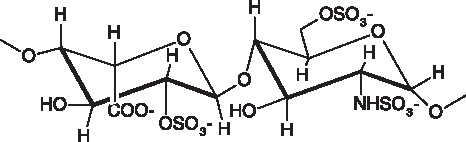
\includegraphics[width=1.0\textwidth]{gfx/background/hp_repeating_unit_structure_01.pdf}
\caption[]{
bla bla bla
}
\label{fig:bg:heparin_chemstruct}
\end{figure}


Most glycosaminoglycans can be found in large quantities in specific cell structures called proteoglycans. These large structures consist of a linear core protein with many glycosaminoglycans covalently linked to it. Each glycosaminoglycan is linked to the core protein via a Gal-Gal-Xyl sugar linker, where the xylose (Xyl) is attached to a serine residue of the core protein and the glycosaminoglycan is linked to the galactose (Gal) residue. Also proteoglycans are highly diverse; variations occur both in the type of core protein and in type, size and number of glycosaminoglycans.



In organisms, GAG chains usually
appear covalently bound to a core protein, comprising a proteoglycan complex.
To a large extent, the biological functions of proteoglycans depends on the
interaction of its GAG chain(s) with other proteins.



Considering the level of atomic detail aimed for ... to be observed... in this
thesis project, GAGs are modeled as short molecules. While it is likely
that their tremendous length and also their covalent linkage to proteoglycans
serve have an overall impact on the biological function of GAGs, it is a
valid and well-established approximation to not account for these facts in
molecular modeling studies that aim for resolving the molecular mechanism of
protein-GAG interaction in atomic detail... in a biological function and overall  treated as


are play a critical role in many biological processes.
Their multifarious biological activity arises from their ability to interact
with and regulate a large number of proteins.


Glycosaminoglycans (GAGs) play a critical role in many biological processes.
Their multifarious biological activity arises from their ability to interact
with and regulate a large number of proteins \cite{handel_2005}.

Introduce abbreviations (HP, HA, CS4, CS6, dpX, etc.)


degree of polymerization


The origin and geometry of various pyranose monosaccharide conformations is
comprehesibly classified and discussed in
\cite{classification_pyranose_conformers_1960}. The conformational nomenclature
used throughout this thesis follows IUPAC rules, which are well-described in
\cite{iupac_gag_conformations_1980}.


\section{A primer on IL-10 biology}

 IL-10's biological function is mainly considered to be
, but

 has pleiotropic effects in immunoregulation and
inflammation.


        in closing remarks, relate to extracellular matrix


\section{Interleukin-10 (IL-10), and its relation to GAGs}


 anti-inflammatory

- Relevance of IL-10 in immune regulation
- Bio-relevant IL-10-GAG interaction? Motivated by Salek ardakini.

We are interested in GAG interaction with the cytokine interleukin-10 (IL-10,
reviewed in \cite{moore_2001}), which is generally considered to exert an
immunosuppressive function. From \textit{in vitro} experiments, IL-10 is known
to bind GAGs and there is evidence that GAGs may modulate its biological
function \cite{salek_ardakani_2000}. So far however, no structural detail about
IL-10-GAG interaction is known.


Wherever IL-10 is supposed to
regulate an immune response, for instance in the process of wound healing and
tissue regeneration, GAGs are


\section{In-silico methods for investigating receptor-ligand interaction}

\subsection{A primer on docking methods}


    - Methods applied in literature: a mini review
        AutoDock3 stands out, just by experience, not by concept
    - Problems of different complexity: local vs. global docking.
    - (AutoDock 3 protein-GAG blind docking validation study,
        Method, results, discussion, conclusion)

\lipsum[1-5]

\subsection{A primer on molecular dynamics simulations}

\lipsum[1-5]

\subsubsection{End-point free energy methods (\enquote{MM-PB(GB)SA})}
% This label is required in DMD chapter.
\label{methods:mmpbsa_mmgbsa}


Cite this: \cite{schlick_innovationsdynamics_2012} (volume 2, chapter 12).

\lipsum[1-5]

\section{Structure of IL-10 and its receptors}

    - Structure description
        exists mainly as homodimer [
            biochemistry, 1998, 37, 16943-16951, zdanov 1995]


    - IL-10 and its receptors
        - what is known in literature (current state of knowlege)
            R1+IL-10 structure
            R2 structure
            ternary complex binding models
            what is required for signaling? literature overview
        - a critical review: monomer
            minimal unit required for signaling (monomer)
        - IL-10 + R1 + R2 structure model from IL20 ternary complex


\section{Aim and scope of this thesis}

- Vision: gaining control over IL-10 function in artificial extracellular matrices

- Motivation and goal: investigate IL-10-GAG system with computational
      methods, in collaboration with...

The aim of this project is to unravel atomic details of IL-10-GAG interaction
with theoretical and computational means. If required, methodological approaches
are to be developed. Integration of \textit{in silico}-based predictions with
experimental results from collaborators will hopefully provide insights into the
mechanisms determining IL-10-GAG interaction. Methodology developed during this
project is applicable to protein-GAG systems in general, rendering it valuable
for a large field of research.



\hl{cite interleukin-2 -heparin interaction (mulloy, rider) !}

\lipsum[1-5]





